\documentclass{siproblemset}

% SI Session Information
\course{MTH 1321}       % the course of your SI
\sessionnum{16}         % (optional) specify the session number
\sessiondate{3/31/20}   % the date of the session

\warmup{Concept Review}
\topic{Concavity}
\topic{Points of Inflection}
\topic{Second Derivative Test}
\cooldown{Extrema from Graphs}

% Worksheet Information
\title{The Second Derivative\linebreak Test and Concavity}
\sections{Section 4.4}
\withnamespace

\begin{document}
    \maketitle
    
    \activity{Activity 1}{Second Derivative Test}{Make a \textbf{group of two or three, all with the same colored worksheets,} to answer your assigned question. Then, try to answer the other questions. Try not to use your notes.}{30 minutes}
    
    \mcq{For the following functions, (a) find the critical points and, (b) if possible, use the Second Derivative Test to classify them as local minimums, local maximums, or neither. If the Second Derivative Test is inconclusive, state so explicitly and use another method.}{
        \task $f(x)=2x^4-3x^2+2$
        \largesp
        \task $g(x)=(x^2-2)e^{-x}\hspace{0.5cm}$
    }
    \newpage

    \activity{Activity 2}{Concavity and Points of Inflection}{Make a \textbf{group of two or three, all with different colored worksheets,} to answer your assigned question. Then, try to answer the other questions. Try not to use your notes.}{30 minutes}
    
    \mcq{For the following functions, (a) find the inflection points and, (b) determine the intervals of concavity.}{
        \task $f(t)=t^3-6t^2+4$
        \Largesp
        \task $y=\theta-2\sin\theta\hspace{0.5cm}[0, 2\pi]$

    }
\newpage
    
    
    \mcq[2]{The following graph is the graph of $f'$, the derivative of the twice-differentiable function $f$. Determine the following:}{
        \task The $x$-values of local extrema
        \task The $x$-values of inflection points
        \task Intervals of increase and decrease of $f$
        \task Intervals where $f$ is concave up and down
    }
    
    \begin{center}
        \mbox{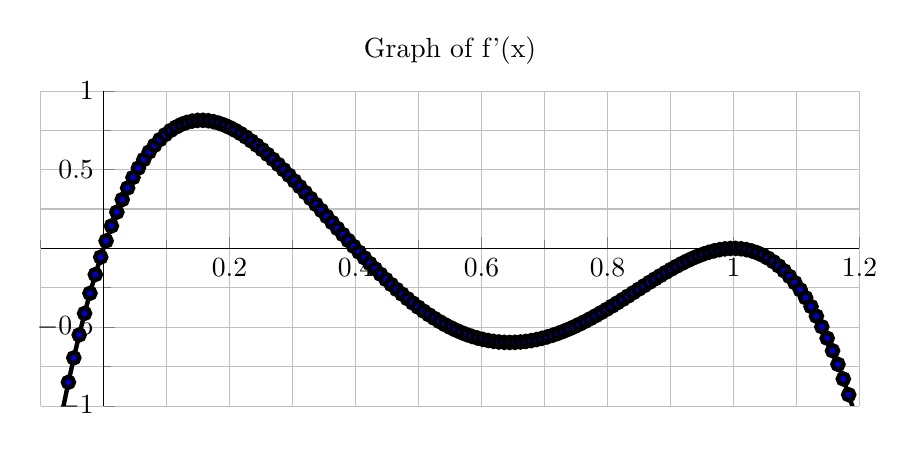
\begin{tikzpicture}[baseline=(current bounding box.north)]
            \begin{axis}[
            title={Graph of f'(x)},
            x=8cm,
            y=2cm,
            xmin=-0.1,
            xmax=1.2,
            ymin=-1,
            ymax=1,
            grid=both,
            major grid style={line width=.2pt,draw=gray!50},
            minor tick num=1,
            axis x line*=middle,
            axis y line*=middle,
            every axis plot/.append style={ultra thick},
            samples=200
            ]
            \addplot+[black, domain=-0.5:1.2] {-30*x*(x-0.4)*(x-1)^2};
            \end{axis}
            \end{tikzpicture}}
    \end{center}

\newpage
    
    \activity{Cooldown}{Determining the Behavior of a Function from a Table}{Do this problem \textbf{alone}.}{15 minutes}
    
    Use the table below to answer questions 1-5.
    
    \begin{center}
        \begin{tabular}{|c|c|c|c|c|c|c|c|}
            \hline
            $x$ & 1 & 2 & 3 & 4 & 5 & 6 & 7 \\
            \hline
            $f(x)$ & -3 & 0 & 4 & -2 & 9 & 2 & -4 \\
            \hline
            $f'(x)$ & -3 & 1 & 0 & DNE & 2 & 0 & -1 \\
            \hline
            $f''(x)$ & 3 & 0 & 2 & 1 & 0 & -1.5 & -3\\
            \hline
        \end{tabular}
    \end{center}
    
    \frq{What are the critical points of $f$?}
    \tinysp
    \frq{What are the intervals of increase and decrease?}
    \tinysp
    \frq{What are the intervals of concavity?}
    \tinysp
    \frq{What are the minimums and maximums?}
    \tinysp
    \frq{What are the points of inflection?}
    \tinysp
    
\end{document}